\documentclass[12pt]{article}
\usepackage{graphicx}
\usepackage{caption}
\usepackage{amsmath}
\usepackage{geometry}
\usepackage{float}
\usepackage{booktabs}
\usepackage{longtable}
\usepackage{setspace} % for spacing control
\usepackage{indentfirst}
\usepackage{titlesec}
\setstretch{1.0}       % single line spacing (default)
\setlength{\parskip}{0pt}   % no space between paragraphs
\setlength{\parindent}{0em} % set indentation amount

\geometry{margin=1in}
\setlength{\parskip}{0em}
\setlength{\parindent}{0pt}

\title{Assignment 1 \\ \large Computational Plasticity (SoSe25)}
\author{Bagus Alifah Hasyim \\ 108023246468 \\ Last Three Digits: 468}
\date{}

\begin{document}
\maketitle

\section*{Given Data}
\hspace*{2em}In this section we need to define every data that is given in the assignment, such as the material properties, geometry, 
and other relevant parameters that are needed for the analysis. Therefore, following data shall we define using the author's "immatrikulation nummer":

\begin{itemize}
    \item $E_a = 200 + (10 \times 4) = 240 \;\text{GPa}$  
    \item $\sigma_a = 300 + (10 \times 6) = 360 \;\text{MPa}$
    \item $\sigma_{yb} = 200 + (10 \times 8) = 280 \;\text{MPa}$
\end{itemize}

\section{Introduction}
\hspace*{2em}In this assignment, we will analyze the mechanical response of a baseline plate
and a plate with a circular inclusion under uniaxial loading. 
The analysis will include comparison of obtaining stress-strain curves between the force-displacement and
direct stress-strain curves, differentiating plane stress and plane strain conditions, comparing 
local stress field distribution based on different constitutive models, and evaluating stress at specific points based on mesh sizes.

\hspace*{2em}For the following sections we will systematically address each question in the assignment, 
providing detailed explanations, derivations, and relevant figures or tables to 
support the analysis. 
All calculations and results are based on the provided data and the author's unique 
identification number. Numerical analysis will be performed using Abaqus CAE with an appropriate
boundary condition and settings. 

\section{Set up of the Model}
\hspace*{2em}For the model setup, we will use Abaqus CAE to create a 2D planar-deformable shell model of the plate with the specified geometry, boundary condition, material properties, and mesh.  
\subsection{Geometry and Boundary Conditions}
%add axis in the figure, for direction 1, 2, and 3
\begin{enumerate}
     \item \textbf{Baseline Plate:} A rectangular plate with length $L = 40 \;\text{mm}$, width $W = 10 \;\text{mm}$, and thickness $t = 1 \;\text{mm}$.
        \begin{figure}[H]
        \centering
            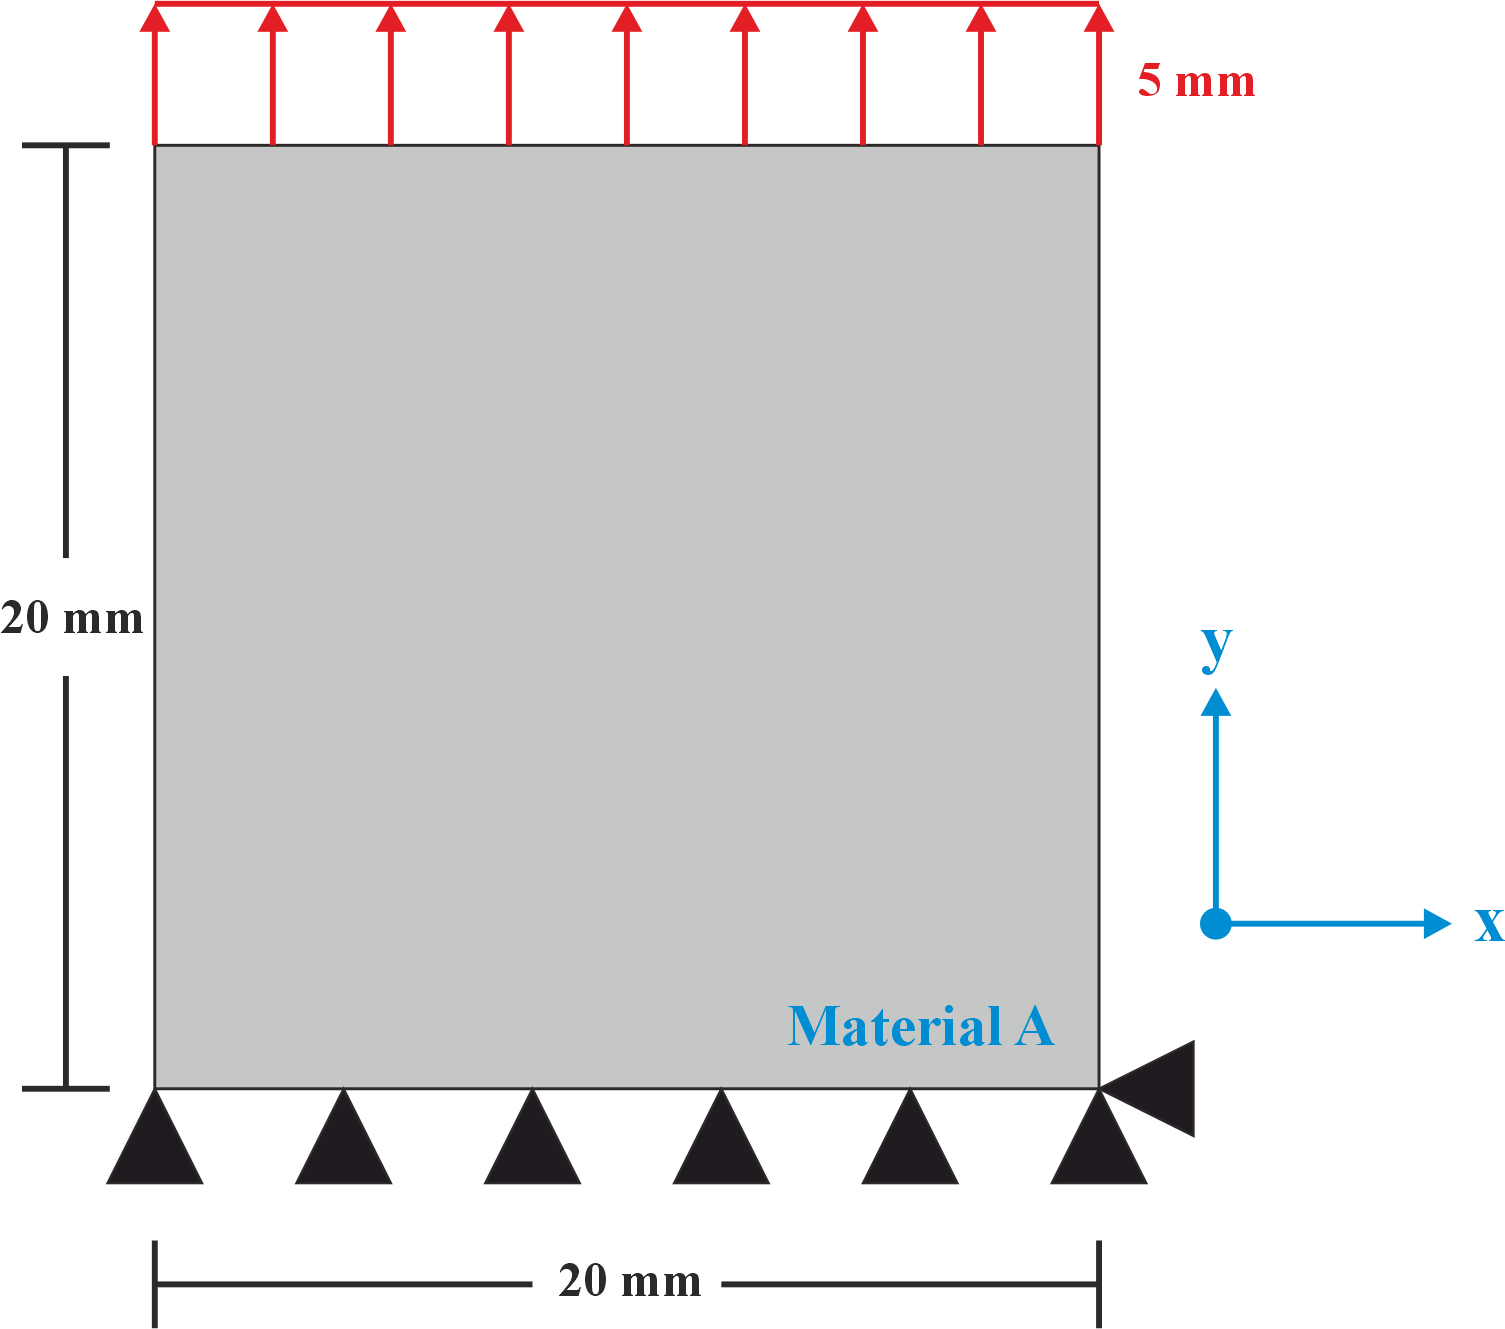
\includegraphics[width=0.5\textwidth]{images/TaskQ1.png}
        \caption{Baseline plate geometry with defined material A. Two boundary conditions are applied, which are the 
        fixed support restriction in y direction on the bottom line of the plate, fixed support point on the bottom right point,
        and constant distribution of displacement in y direction on the top line of the plate, which has value of 5 mm.}
        \label{fig:geometryQ1}
\end{figure}

    \item \textbf{Plate with Circular Inclusion:} Same as the baseline plate, but with a circular inclusion of radius $r$ located at the center or specified position.
\begin{figure}[H]
        \centering
            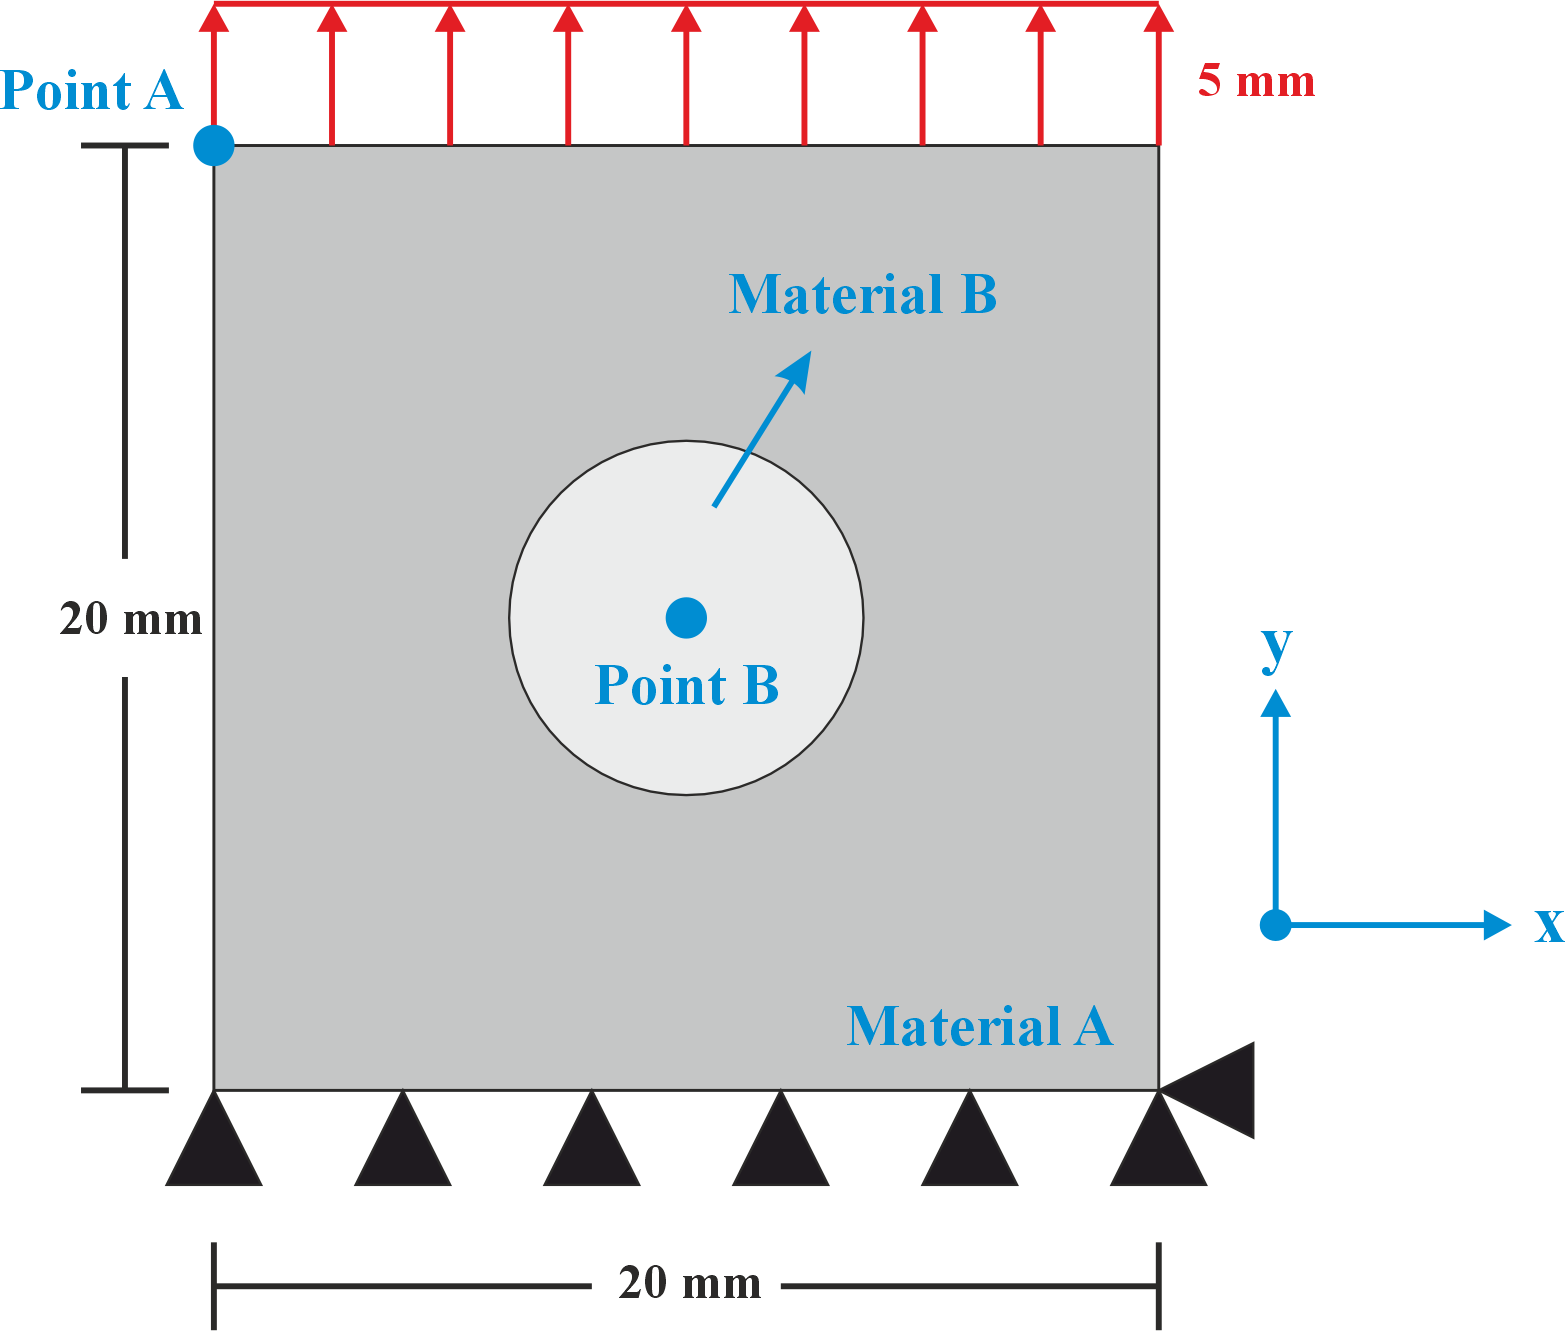
\includegraphics[width=0.52\textwidth]{images/TaskQ2.png}
        \caption{Plate with circular inclusion and defined material B. Boundary conditions are the same as in Task 1 shown in Figure~\ref{fig:geometryQ1}.}
        \label{fig:geometryQ2}
\end{figure}
\end{enumerate}
\subsection{Material Properties}
\hspace*{2em}Material properties for the analysis are provided from the task definition, which there are some
material parameters that need to be manually calculated based on the author's Immatrikulation Nummer in at very 
first section. 
For task 1, material A (see Table~\ref{tab:materialA-properties}) will be used and defined as an elastic-plastic material with properties based on the Young's modulus $E$, Poisson's ratio $\nu$, and yield stress $\sigma_{ya}$,
and ultimate tensile strength $\sigma_{f}$, and the strain at fracture $\epsilon_{f}^{f}$ in isotropic condition.   
For task 2 with additional inclusion material B in the center, it is defined as an elastic-plastic material with anisotropic properties, 
which it defines the properties differently in three orthogonal directions. Especially for the plastic properties in table~\ref{tab:materialB-plasticproperties},
it used Hill's yield criterion, which is defined by the Hill's coefficients $R_{ij}$, where $i,j = 1,2,3$ for the three orthogonal directions. 


\begin{table}[H]
    \centering
    \caption{Elastic and plastic properties of material A.}
    \label{tab:materialA-properties}
    \begin{tabular}{lllll}
        \toprule
        E (GPa) & $\nu$ & $\sigma_{ya}$ (MPa) & $\sigma_{f}$ (MPa) & $\epsilon_{f}^{f}$ \\
        \midrule
        240 & 0.3 & 360 & 550 & 0.4 \\
        \bottomrule
    \end{tabular}
\end{table}

\begin{table}[H]
    \centering
    \caption{Elastic properties of material B.}
    \label{tab:materialB-elasticproperties}
    \begin{tabular}{lllllllll}
        \toprule
            \centering $E_1$ (GPa) & $E_2$ (GPa) & $E_3$ (GPa) & $\nu_{12}$ & $\nu_{13}$ & $\nu_{23}$ & $G_{12}$ (MPa) & 
            $G_{13}$ (MPa) & $G_{23}$ (MPa) \\
            \midrule
            \centering 210 & 220 & 230 & 0.3 & 0.31 & 0.32 & 80 & 84 & 87 \\
            \bottomrule
    \end{tabular}
\end{table}

\begin{table}[H]
    \centering
    \caption{Plastic properties of material B.}
    \label{tab:materialB-plasticproperties}
    \begin{tabular}{lllllllll}
        \toprule
            \centering $R_{11}$ & $R_{22}$ & $R_{33}$ & $R_{12}$ & $R_{13}$ & $R_{23}$ & $\sigma_{yb}$ & 
            $\sigma_{f}$ (MPa) & $\epsilon_{p}^{f}$  \\
            \midrule
            \centering 1 & 1.2 & 1.25 & 0.8 & 0.85 & 0.95 & 280 & 450 & 0.5 \\
            \bottomrule
    \end{tabular}
\end{table}
\subsection{Meshing}
\hspace{2em}The models for this tasked are differentiate into two different 
meshes types, which first one is the homogeneous baseline plate 
with a uniform mesh size distribution, and the 
second one is the plate with circular inclusion,
which it has a customized mesh distribution in order to 
take account creating symmetrical meshes distribution 
across the geometry variant. Creating meshes for geometry with inclusion
should be taking care of some aspects, for instance, defining the distribution 
pattern of the mesh size, which the program mesh algorithm from Abaqus
CAE can automatically generate a symmetrical mesh distribution. Hence, 
defining geometry partition is having an important role in order to achieve
a good mesh distribution. The following figures show the meshing
for both models. Noted that in this assignment, we will not use the
reduced integration element, which in the end the logaritihmic strain
will be shown instead of the regular strain. 
\begin{figure}[H]
    \centering
    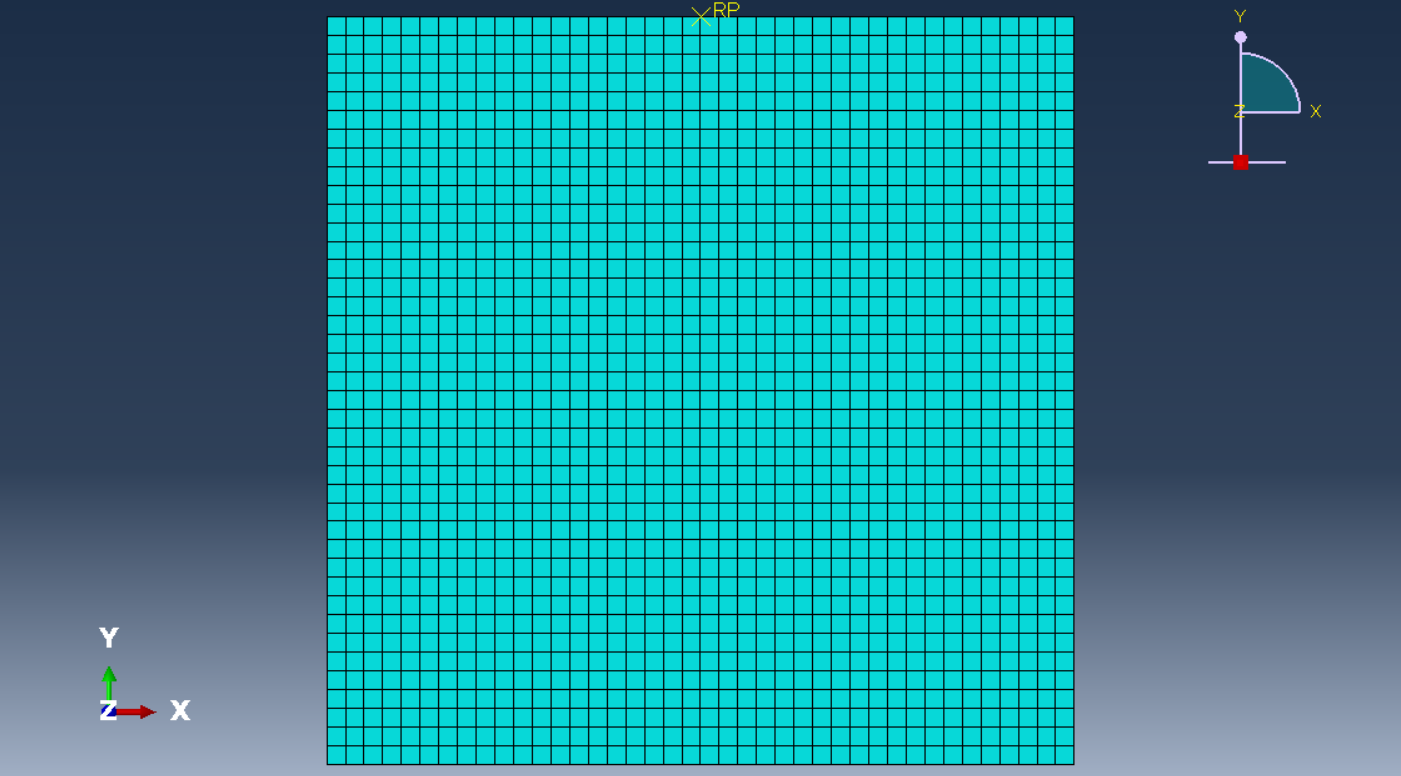
\includegraphics[width=1\textwidth]{images/MeshQ1.png}
    \caption{Mesh for the baseline plate with uniform mesh size distribution, 
    with total of 1600 elements. The mesh size is defined as 0.25 mm
    gap size with set up for both plane stress and plane strain
    conditions.}
    \label{fig:MeshQ1}
\end{figure}

\begin{figure}[H]
    \centering
    \begin{minipage}{0.48\textwidth}
        \centering
        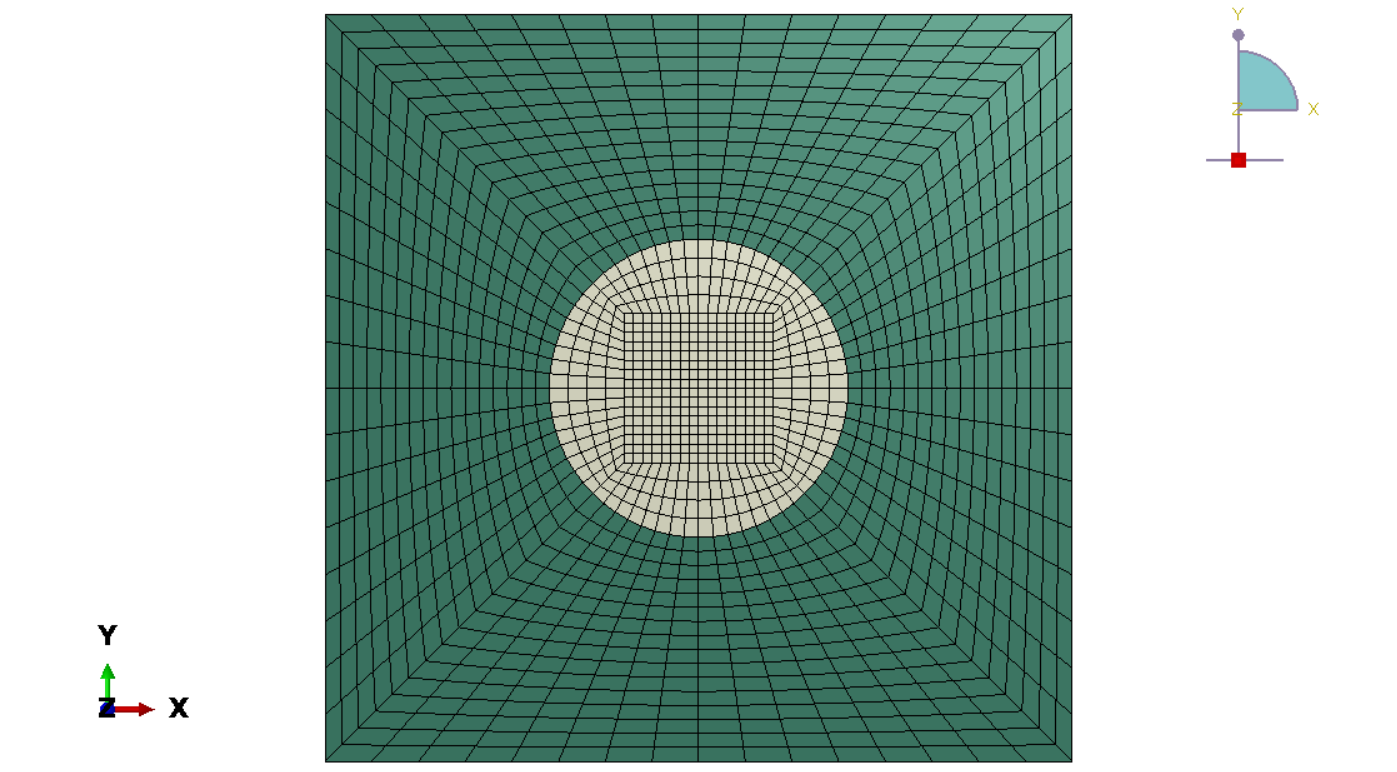
\includegraphics[width=\textwidth]{images/MeshQ2.1.png}
        \caption{Mesh for the plate with circular inclusion for the coarse variation
        with 1536 elements.}
        \label{fig:MeshQ2.1}
    \end{minipage}\hfill
    \begin{minipage}{0.48\textwidth}
        \centering
        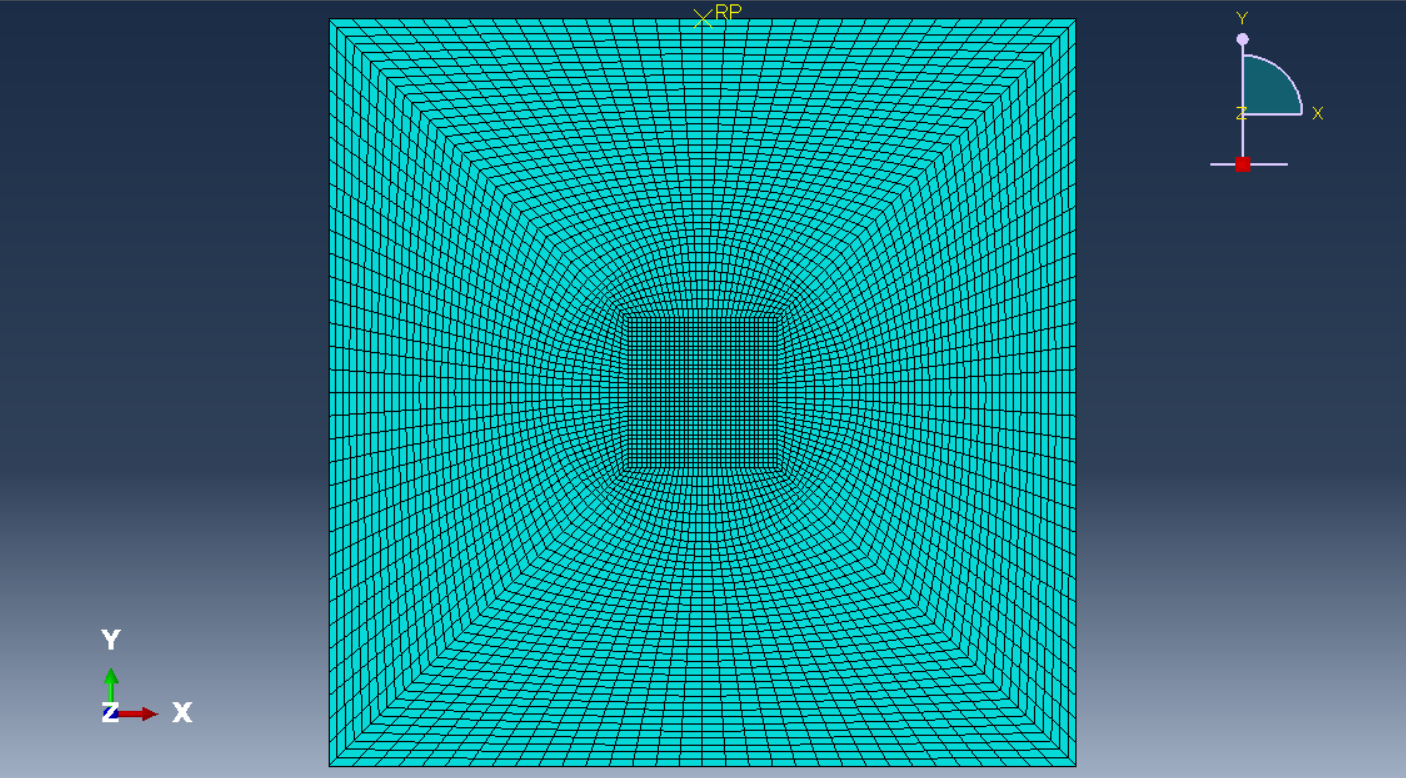
\includegraphics[width=\textwidth]{images/MeshQ2.2.png}
        \caption{Mesh for the plate with circular inclusion for fine mesh variation
        with 6144 elements.}
        \label{fig:MeshQ2.2}
    \end{minipage}
\end{figure}
\section*{Results and Discussion}

\subsection*{Q1: Mechanical Response Analysis for Baseline Plate}
\begin{figure}[H]
    \centering
    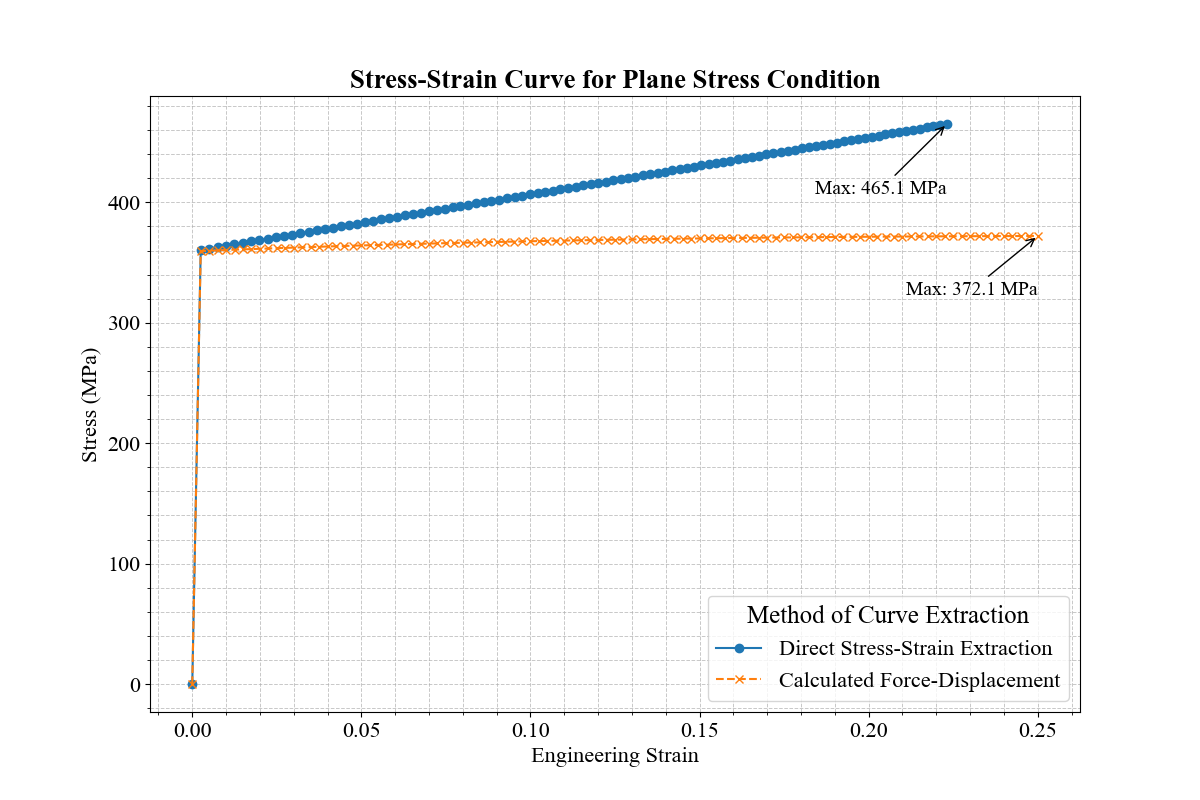
\includegraphics[width=1\textwidth]{visualize_tensileGraph/res/comparison_direct_calculated.png}
    \caption{Comparison of
    the stress-strain curves obtained from the force-displacement method and the direct stress-strain calculation
    for plane stress condition. The direct stress-strain curve method is obtained 
    by extracting the stress $\sigma_{22}$ and strain $\varepsilon_{22}$ directly from the 
    history output, which are the whole nodes along the top edges of the baseplate. While the caculated
    Force-Displacement is obtained by extracting the force 
    $F_{22}$ and displacement $U_{22}$ from the history output, which are the whole nodes along the top edges of the baseplate.
    Then the stress is obtained by dividing the force with the surface area
    normal to the loading direction, which are 20 $mm^2$ 
    \label{fig:ComparisonDirectCalculated}  
\end{figure}

\subsection*{Q2: Mechanical Response Analysis for Plate with Circular Inclusion}
XXX…

\subsection*{Q3: Local Stress Field Distribution and Analysis}
XXX…

\subsection*{Q4: Comparison Analysis at Point A}
XXX…

\subsection*{Q5: Comparison Analysis at Point B}
XXX…

\subsection*{Extra Task}
To calculate $\frac{\partial{f}}{\partial{\sigma}}$ with Voigt notation tensor $\sigma = (\sigma_1, \sigma_2, \sigma_3, \sigma_4, \sigma_5, \sigma_6)$ from yield function 
$f(\sigma)=\sigma_{eq} - \sigma_y$, where $\sigma_{eq}$ can be described as follows:

\begin{equation}
\sigma_{eq} = \sqrt{\frac{1}{2} \left( (\sigma_1 - \sigma_2)^2 + (\sigma_2 - \sigma_3)^2 + (\sigma_3 - \sigma_1)^2 + 6(\sigma_4^2 + \sigma_5^2 + \sigma_6^2) \right)}
\end{equation}

Hence, we can simplify the prescribed equation to:

\begin{equation}
A = \frac{1}{2} \left( (\sigma_1 - \sigma_2)^2 + (\sigma_2 - \sigma_3)^2 + (\sigma_3 - \sigma_1)^2 + 6(\sigma_4^2 + \sigma_5^2 + \sigma_6^2) \right)
\end{equation}

We can substitute the equation above into the yield function $f(\sigma)$ and applying the chain rule in the 
derivative, we obtain:

\begin{equation}
f(\sigma) = \sqrt{A} - \sigma_y \rightarrow \frac{\partial{f}}{\partial{\sigma}} = \frac{\partial{f}}{\partial{A}} \cdot \frac{\partial{A}}{\partial{\sigma}} = \frac{1}{2\sqrt{A}} \cdot \frac{\partial{A}}{\partial{\sigma}}
\end{equation}

Since we defined $A$ as a substituent of the equivalent stress $\sigma_{eq}$, we can revert the equation as in the origin form:

\begin{equation}
    \frac{\partial{f}}{\partial{\sigma}} = \frac{1}{\sigma_{eq}} \cdot \frac{\partial{A}}{\partial{\sigma}}
\end{equation}

Now we need to expand the tensor differential with respect to each stress component in 
the Voigt notation. Therefore, we can do the differential operation for each stress 
component and assemble them to a Voigt notation as following sequence:

\[
\frac{\partial{A}}{\partial{\sigma_1}} = H_{1}(\sigma_1-\sigma_2) + H_3(\sigma_1-\sigma_3) \;;
\]
\[
\frac{\partial{A}}{\partial{\sigma_2}} = H_{2}(\sigma_2-\sigma_3) + H_1(\sigma_2-\sigma_1) \;;
\]
\[
\frac{\partial{A}}{\partial{\sigma_3}} = H_{2}(\sigma_3-\sigma_2) + H_3(\sigma_3-\sigma_1) \;;
\]
\[
\frac{\partial{A}}{\partial{\sigma_4}} = 6H_{4}\sigma_4 \;;
\]
\[
\frac{\partial{A}}{\partial{\sigma_5}} = 6H_{5}\sigma_5 \;;
\]
\[
\frac{\partial{A}}{\partial{\sigma_6}} = 6H_{6}\sigma_6 \;;
\]

To summarize the above equations, we can write them in a matrix form as follows:
\begin{equation}
\frac{\partial{f}}{\partial{\sigma}} = \frac{1}{\sigma_{eq}}\begin{bmatrix}
H_{1}(\sigma_1-\sigma_2) + H_3(\sigma_1-\sigma_3) \\    
H_{2}(\sigma_2-\sigma_3) + H_1(\sigma_2-\sigma_1) \\
H_{2}(\sigma_3-\sigma_2) + H_3(\sigma_3-\sigma_1) \\
6H_{4}\sigma_4 \\
6H_{5}\sigma_5 \\
6H_{6}\sigma_6
\end{bmatrix}
\end{equation}




\section*{Conclusion}
(Summarize your findings and state key takeaways from the analysis)



\end{document}

